\documentclass[a4paper,11pt, twocolumn]{article}
\usepackage[margin=0.8in]{geometry}
\usepackage{xcolor}
\usepackage{graphicx} %package to manage images
\graphicspath{ {./images/} }
\usepackage{float}
\usepackage{fancyvrb}
\usepackage{fvextra}
\usepackage{tabularx}

\title{1.4.2 Data Structures}
\author{Revision sheet}
\date{}

\usepackage{fancyhdr}
\pagestyle{fancy}
\fancyhead{} % clear all header fields
\renewcommand{\headrulewidth}{0pt} % no line in header area
\fancyfoot{} % clear all footer fields
\renewcommand{\footrulewidth}{0.4pt}
\fancyfoot[C]{\thepage} % page number in centre of the page
\fancyfoot[R]{\footnotesize Thomas Boxall \\ Some images from Physics And Maths Tutor} % right hand footer has author name on top line and images reference on bottom line
\fancyfoot[L]{\footnotesize 1.4.2 Data Structures \\ Revision sheet} % left hand footer has title of document on top line and 'Revision Sheet' on bottom line


\begin{document}

\maketitle
\thispagestyle{fancy}

% CONTENTS OF THE REVISION SHEET HERE
\section{Arrays}
\textit{A data structure for storing a finite, ordered set of data of the same data type within a single identifier.}\\
Arrays come in up-to three dimensions. They are all fundamentally the same.
\subsection{1-Dimensional Array}
\begin{figure}[H]
    \centering
    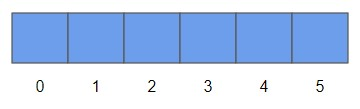
\includegraphics[width=0.45\textwidth]{1dArray.jpg}
    \label{fig:1dArray}
    \caption{1D Array}
\end{figure}
\noindent The one-dimensional array is based off of a 0 based index. The pseudocode below shows how you can set the contents of the array and how to access one of the indexes.
\begin{Verbatim}[breaklines=true, breakanywhere=true]
oneDimensionalArray = [1, 23, 12, 14, 16, 55]
print(oneDimensionalArray[3]) //outputs 14
\end{Verbatim}
\subsection{2-Dimensional array}
\begin{figure}[H]
    \centering
    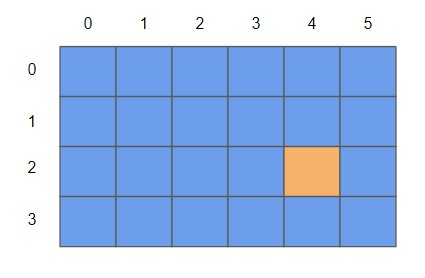
\includegraphics[width=0.45\textwidth]{2dArray.jpg}
    \label{fig:2dArray}
    \caption{2D Array}
\end{figure}
\noindent Two-Dimensional arrays are declared in a similar way to that of a 1D array.
\begin{Verbatim}[breaklines=true, breakanywhere=true]
twoDimensionalArray = [[1, 23, 12, 14, 16, 55], [2, 56, 67, 23, 11, 89], [23, 12, 114, 64, 25, 65], [97, 65, 16, 13, 36, 56]]
print(twoDimensionalArray[1,3]) //down then across. Outputs 23
\end{Verbatim}
For the diagram shown in Figure \ref{fig:2dArray}, the orange square would be at location \verb|[2,4]| as the indexes are addressed down then across.
\subsection{3-Dimensional Arrays}
3D arrays can be visualised as a multi-page spreadsheet, and can be thought of as multiple 2D arrays. 
\begin{figure}[H]
    \centering
    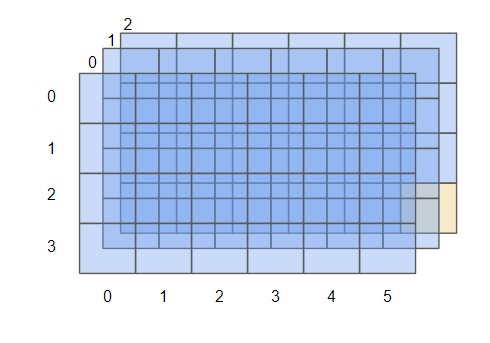
\includegraphics[width=0.45\textwidth]{3dArray.jpg}
    \label{fig:3dArray}
    \caption{3D Array}
\end{figure}
\noindent Three-Dimensional arrays are declared in much the same way as two dimensional arrays, except there are multiple 2D arrays in the same declaration.
\begin{Verbatim}[breaklines=true, breakanywhere=true]
threeDimensionalArray = [[[12,8],[9,6,19]],[[241,89,4,1],[19,2]]]
print(threeDimensionalArray[0,1,2]) //outputs 19
\end{Verbatim}
For the diagram shown in Figure \ref{fig:3dArray}, the orange square would be at location \verb|[2,3,5]| as the it is [arrayNumber, rowNumber, columnNumber].

\section{Tuples}
\textit{A data structure for sorting an immutable (cannot be modified once created), ordered set of data, which can be of different data types, within a single identifier.}\\
Tuples are initialised using regular brackets instead of square brackets:
\begin{Verbatim}[breaklines=true, breakanywhere=true]
tupleExample = ("Value1", 2, "Value3") 
print(tupleExample[0]) //outputs "Value1"
\end{Verbatim}

\section{Records}
\textit{A data structure that stores data in elements called fields, organised based on attributes.}\\
\begin{figure}[H]
    \centering
    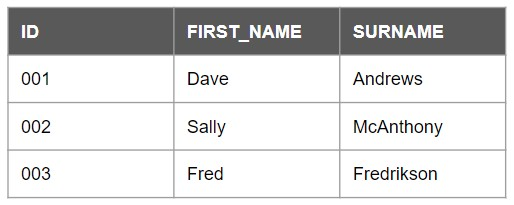
\includegraphics[width=0.45\textwidth]{record.jpg}
    \label{fig:record}
    \caption{Record}
\end{figure}
\noindent The pseudocode below would be used to declare the record shown in Figure \ref{fig:record}.
\begin{Verbatim}[breaklines=true, breakanywhere=true]
    pupilDataType = record
    integer ID
    string FIRST_NAME
    string SURNAME
end record
\end{Verbatim}
Each field in the record can be identified by \verb|recordName.fieldName|. The variable which holds the record is declared as \verb|pupil1 : pupilDataType|

\section{Linked Lists}
\textit{A data structure that stores an ordered sequence of data where each item is stored with a pointer to the next item. The items are not stored contiguously (in the same order) in memory.}\\
Linked lists are dynamic.
\begin{figure}[H]
    \centering
    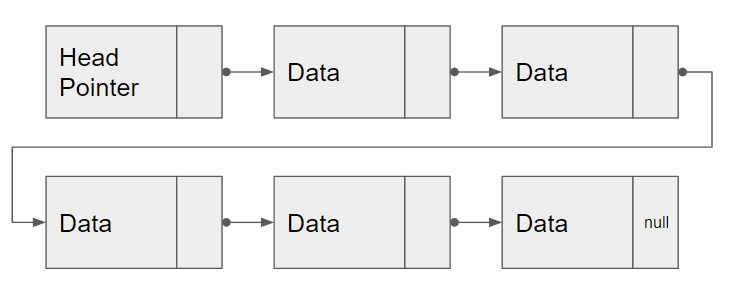
\includegraphics[width=0.45\textwidth]{linkedList.jpg}
    \label{fig:linkedList}
    \caption{Linked List}
\end{figure}
\noindent Linked lists are good because they can grow according to the needs of the user and it is easier to insert a new element (you just insert it at any point in memory and update the relevant pointers). To search a linked list, you have to start at the head pointer and work through every element until you either reach the end or find the item you are looking for. This can take some time if you have a very long linked list. Due to it not being stored contiguously in memory, there is no random access, to find any elements you have to search as described above.\\
Linked lists could be implemented in an object oriented approach with attributes for the index (memory location), data and pointer to the next index.

\section{Hash Tables}
\textit{A data structure where a hashing algorithm calculates a value to determine where a data item is to be stored. The data item can then be directly accessed by recalculation, without any search.}\\
These are often implemented as an array. A good hashing algorithm would have a low possibility of a collision occurring; if a collision does occur, it will need to be resolved. There are two ways in which collisions can be resolved.
\paragraph*{Linear probing} If the address is already full, then you move through the table 1 index at a time to find a free space. The data is put in the first free space found. Advantages: can use less memory; can perform faster; if there isn't a collision, the data is placed in the first place you look.
\paragraph*{Chaining} Each location points to a linked list. New items are inserted into the linked list. When searching, you go through the linked list to find the item. Advantage: no limit on the amount of data that can be stored.
\paragraph*{Overflow area} There is an overflow area setup at the bottom of the table, any collisions get dumped in the overflow area. Disadvantage: really inefficient as to find an item, you might have to look through all of the overflow area, which could be massive.

\section{Stack}
\textit{A last-in-first-out (LIFO) data structure. The last item added/pushed is the first item to be removed/popped off.}\\
Stacks can either be static or dynamic and are often implemented using one directional arrays, with additional pointers for current top item or next free slot, max size.
\begin{figure}[H]
    \centering
    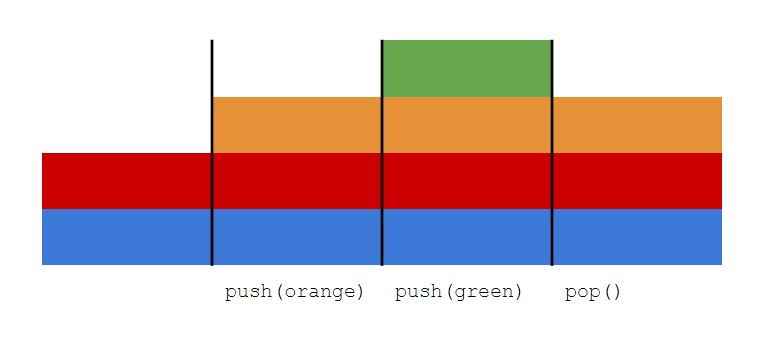
\includegraphics[width=0.45\textwidth]{stack.jpg}
    \label{fig:stack}
    \caption{Stack}
\end{figure}
\noindent Variables which are in memory are loaded onto a stack when a function is called. 

\section{Queues}
\textit{A first-in-first-out (FIFO) data structure. The first item enqueued on to the queue is the first to be dequeued off of the queue.}\\
Queues can either be circular or linear. Queues can be implemented in an array. Alongside the array, you will need a number of pointers: front pointer, rear pointer, max number of elements, number of elements currently in the queue. Queues are static and quite often used in a keyboard buffer. 
\begin{figure}[H]
    \centering
    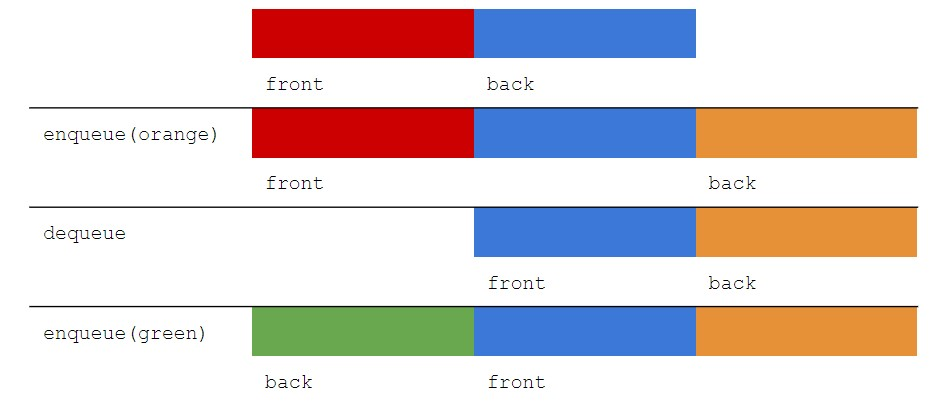
\includegraphics[width=0.45\textwidth]{queue.jpg}
    \label{fig:queue}
    \caption{Circular queue}
\end{figure}
\noindent The diagram above shows how a circular queue works. 

\section{Graphs}
\textit{A data structure consisting of a set of vertices/nodes connected by a set of arcs/edges.}\\
\begin{figure}[H]
    \centering
    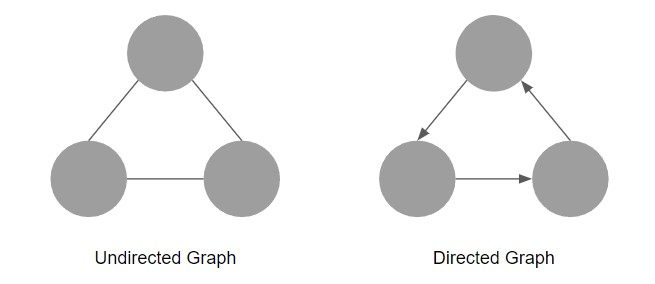
\includegraphics[width=0.45\textwidth]{graphsDirUndir.jpg}
    \label{fig:graphsDirUndir}
    \caption{Undirected and directed graphs}
\end{figure}
\noindent Graphs come in two flavours, directed and undirected. The edges on a directed graph are shown with arrows, whereas on an undirected graph they are plain lines. Edges on a graph can be weighted (shown by a number on the edge). 
\subsection{Storing The Graph}
Graphs can be stored as an adjacency matrix or adjacency list.
\begin{figure}[H]
    \centering
    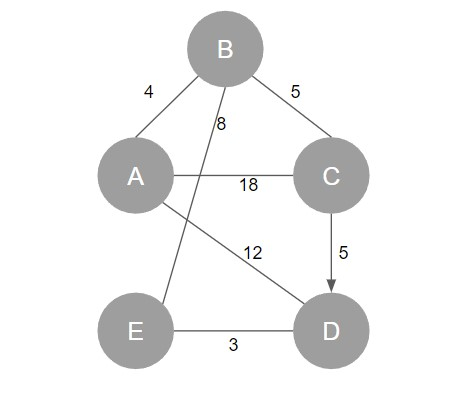
\includegraphics[width=0.45\textwidth]{graphsForEx.jpg}
    \label{fig:grapshForEx}
    \caption{Graphs used for Storage Examples}
\end{figure}
\subsubsection{Adjacency Matrix}
Adjacency matrices can be implemented as a two dimensional array as shown below.
\begin{table}[H]
    \centering
    \begin{tabularx}{0.45\textwidth}{X|XXXXX}
        & A & B & C & D & E\\
        \hline
        A & - & 4 & 18 & 12 & - \\
        B & 4 & - & 5 & - & 8 \\
        C & 18 & 5 & - & 5 & - \\
        D & 12 & - & - & - & 3 \\
        E & - & 8 & - & 3 & - \\
    \end{tabularx}
\end{table}
\noindent The matrix is read down then across. For example traversing from C(down) to D(across) is 5, but traversing from C(across) to D(down) is - as C-D is directed. Adjacency matrices are more convenient to work with as they have shorter access times and are easier to add nodes.
\subsubsection{Adjacency List}
\begin{enumerate}
    \item[A] B:4, C:18, D:12
    \item[B] A:4, C:5, E:8
    \item[C] A:18, B:5, D:5
    \item[D] A:12, E:3
    \item[E] B:8, D:3
\end{enumerate}
Adjacency lists are more efficient for larger, sparser networks.
\subsection{Traversal}
Traversing a graph can either be done breadth-first or depth-first. 
\subsubsection{Breadth-First Traversal}
\paragraph{Used for} finding the shortest path in things like GPS systems; applications like Facebook for keeping track of friends; web crawlers.
\paragraph{Steps}
\begin{enumerate}
    \item Pick one of the graph vertices and put it at the back of the \verb|toVisit| queue.
    \item Take the first item off of \verb|toVisit| and add it to the \verb|visited| list.
    \item Enqueue all children of the current node which aren't in \verb|visited| to \verb|toVisit|.
    \item Keep repeating steps 2 and 3 until \verb|toVisit| is empty.
\end{enumerate}
\subsubsection{Depth-First Traversal}
This can either be pre-order or post-order.
\paragraph{Used for} mazes and job scheduling.
\paragraph{Steps}
\begin{enumerate}
    \item Pick anyone of the graph vertices and push it onto the stack \verb|toVisit|.
    \item Pop the first item off of \verb|toVisit| and add it to \verb|visited|
    \item For the current node, if its children aren't in \verb|visited| push them to \verb|toVisit|.
    \item Keep repeating steps 2 and 3 until \verb|toVisit| is empty.
\end{enumerate}

\section{Trees}
\textit{A data structure that uses a set of linked nodes to form a hierarchical structure starting at a root node. Each node is a child/sub-node of a parent node.}\\
There are two types of trees: binary and non-binary. Fundamentally, all trees are the same.
\begin{figure}[H]
    \centering
    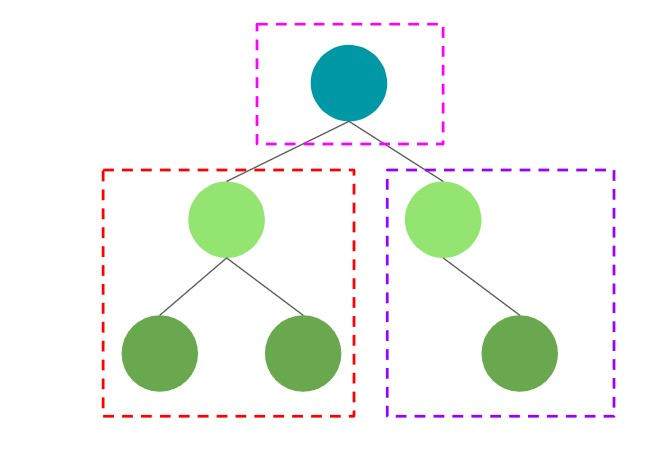
\includegraphics[width=0.45\textwidth]{treeIntro.jpg}
    \label{fig:treeIntro}
    \caption{Basic structure of a tree}
\end{figure}
\noindent The cyan node is called the root node. The light green nodes are parent nodes. The dark green nodes are leaf/children nodes. The red box indicates the left sub tree and the purple box indicates the right subtree.\\
The key difference between a binary and non-binary tree are the number of child nodes a single node can have. In a binary tree, a parent node can only have 0, 1 or 2 child nodes. Whereas in a non-binary tree, a parent node can have any number of child nodes.
\subsection{Traversing a Tree}
There are three different \textit{routes} which can be taken when traversing a tree.
\subsubsection{In Order Traversal}
\begin{figure}[H]
    \centering
    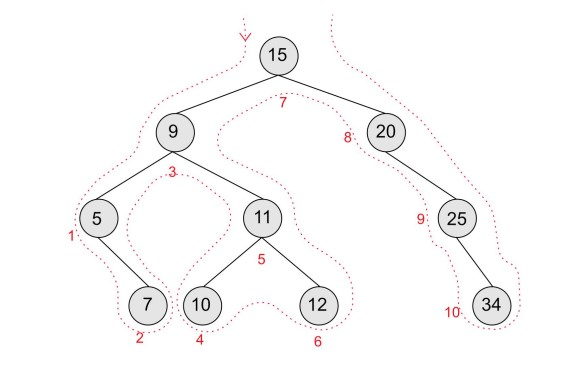
\includegraphics[width=0.45\textwidth]{treeInOrder.jpg}
    \label{fig:treeInOrder}
    \caption{In order traversal route}
\end{figure}
\noindent Traverse: left subtree, root node, right subtree.
\subsubsection{Pre-Order Traversal}
\begin{figure}[H]
    \centering
    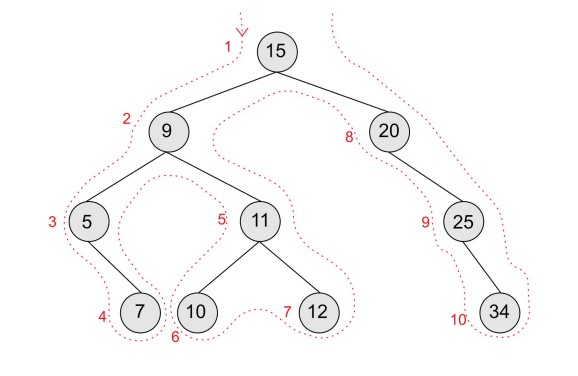
\includegraphics[width=0.45\textwidth]{treePreOrder.jpg}
    \label{fig:treePreOrder}
    \caption{Pre-order traversal route}
\end{figure}
\noindent Traverse: Root node, left subtree, right subtree.
\subsubsection{Post-Order Traversal}
\begin{figure}[H]
    \centering
    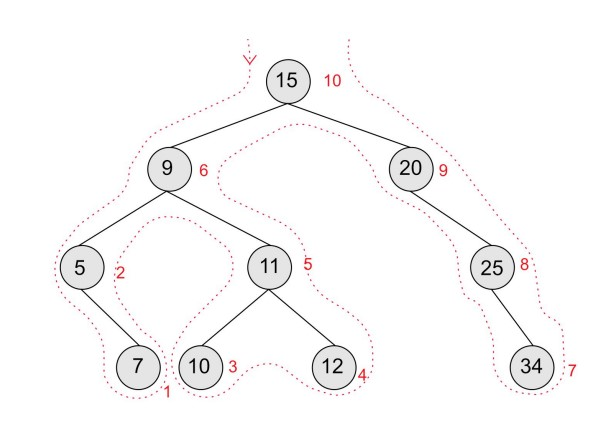
\includegraphics[width=0.45\textwidth]{treePostOrder.jpg}
    \label{fig:treePostOrder}
    \caption{Post order traversal route}
\end{figure}
\noindent Traverse: Left subtree, right subtree, route node.


\end{document}